\documentclass[12pt]{beamer}
\usetheme{jaifat}

\usepackage{hyperref}
\usepackage{setspace}
\usepackage[labelformat=empty]{caption}
\usepackage{ulem}

%% =============
%% new command

\newcommand{\frametitlecenter}[1]{
%\vskip 12mm
\hskip 3mm
\vskip 10mm
% \vskip 18pt
\begin{beamercolorbox}[wd=.8\paperwidth,ht=1.5cm,center]{frametitle}
  \usebeamerfont*{frametitle}{
    \begin{spacing}{1.1} \fontsize{32}{32}\selectfont{#1} \end{spacing}
  }\end{beamercolorbox}
}%

\newcommand{\ftc}[1]{\frame{\frametitlecenter{#1}}}%
\newcommand{\ftcc}[2]{\frame{#2\frametitlecenter{#1}}}%
\newcommand{\jref}[2]{\href{#1}{\underline{#2}}}%

% \renewcommand{\figurename}{}

%% =============
%% meta-data

\title{Implementing Untyped λ-Calculus}
\subtitle{in Haskell}

\author{slide: Jaiyalas \\ Lin Jen-Shin (godfat)}
\date{2012-05-08}

%% =============
%% document body

\begin{document}
\frame{\titlepage}


\section{Who Am I?}

\ftc{Who Am I?}

%\subsection{What I learned?}
%\ftc{What I learned?}
\frame{\frametitle{What I learned?}
\begin{itemize}
\item[] {}
\item {2007$\sim$present: (learning) Haskell}
\item {2006$\sim$present: Ruby}
\item {2005$\sim$2008: C++}
\item {2001$\sim$2004: C}
\item[] {}
\end{itemize}
}

%\subsection{What I worked?}

%\ftc{What I worked?}
\frame{\frametitle{What I worked?}
\begin{itemize}
\item[] {}
\item[] {}
\item roodo.com
\item cardinalblue.com
\item[] {}
\item[] {}
\end{itemize}
}

%\subsection{Where you can find me}

%\ftc{Where you can find me}
\frame{\frametitle{Where you can find me}
\begin{itemize}
\item[] {}
\item \jref{https://github.com/godfat}{github.com/godfat}
\item \jref{https://twitter.com/godfat}{twitter.com/godfat}
\item \jref{https://profiles.google.com/godfat}{profiles.google.com/godfat}
\item[] {}
\item[] {}
\end{itemize}
}

\frame{\frametitle{How I started to learn Haskell}
\begin{itemize}
\item[] {}
\item <1->{PLT at {\usebeamerfont*{font DejaVu Sans Mono}{ssh://bbs@ptt.cc}} }
\item <2->{IIS at Sinica}
\item <3>{FLOLAC}
\item[] {}
\item[] {}
\end{itemize}
}

\section{Who Am I?}

\ftc{Who Am I?}

%\subsection{What I learned?}
%\ftc{What I learned?}
\frame{\frametitle{What I learned?}
\begin{itemize}
\item[] {}
\item {2007$\sim$present: (learning) Haskell}
\item {2006$\sim$present: Ruby}
\item {2005$\sim$2008: C++}
\item {2001$\sim$2004: C}
\item[] {}
\end{itemize}
}

%\subsection{What I worked?}

%\ftc{What I worked?}
\frame{\frametitle{What I worked?}
\begin{itemize}
\item[] {}
\item[] {}
\item roodo.com
\item cardinalblue.com
\item[] {}
\item[] {}
\end{itemize}
}

%\subsection{Where you can find me}

%\ftc{Where you can find me}
\frame{\frametitle{Where you can find me}
\begin{itemize}
\item[] {}
\item \jref{https://github.com/godfat}{github.com/godfat}
\item \jref{https://twitter.com/godfat}{twitter.com/godfat}
\item \jref{https://profiles.google.com/godfat}{profiles.google.com/godfat}
\item[] {}
\item[] {}
\end{itemize}
}

%\subsection{How I started to learn Haskell}

%\ftc{How I started to learn Haskell}
\frame{\frametitle{How I started to learn Haskell}
\begin{itemize}
\item[] {}
\item <1->{PLT at {\usebeamerfont*{font DejaVu Sans Mono}{ssh://bbs@ptt.cc}} }
\item <2->{IIS at Sinica}
\item <3>{FLOLAC}
\item[] {}
\item[] {}
\end{itemize}
}

%%%%%%  section break line %%%%%%

\section{Table of Contents}
%\ftc{Table of Contents}
\frame{\frametitle{Table of Contents}
    \begin{itemize}
      \item {What can Haskell do?}
      \item {What is λ-Calculus?}
      \item {Why Implement λ-Calculus?}
      \item {Let's Implement λ-Calculus}
      \item {Questions?}
      \item {References}
    \end{itemize}
}

%%%%%%  section break line %%%%%%
\section{What can Haskell do?}
%\ftc{What can Haskell do?}
%%%% special case!
% \frame{\vskip 12mm%
% \frametitlecenter{What can\\Haskell do?}
% }
\frame{\frametitle{Table of Contents}
  \begin{itemize}
    \item {What can Haskell do?}
    \item {\color{lightgray} What is λ-Calculus?}
    \item {\color{lightgray} Why Implement λ-Calculus?}
    \item {\color{lightgray} Let's Implement λ-Calculus}
    \item {\color{lightgray} Questions?}
    \item {\color{lightgray} References}
  \end{itemize}
}


\ftc{Defined in 1990}

% \ftc{Successor of Miranda from 1985}
%%%% special case!
\frame{\vskip 22mm%
\frametitlecenter{Successor of Miranda from 1985}
}

\ftc{Haskell 98}

\ftc{Haskell 2010}

%\ftc{GHC (Glasgow Haskell Compiler)}
\frame{\frametitle{GHC (Glasgow Haskell Compiler)}
\begin{itemize}
  \item[]{}
  \item<1->{STM {\normalsize (Software Transactional Memory)}}
  \item<2->{Template Haskell}
  \item<3->{GADT {\normalsize (Generalized Algebraic Data Type)}}
  \item[]{}
  \item[]{}
\end{itemize}
}

%\ftc{Notable Projects}
\frame{\frametitle{Notable Projects}
\begin{itemize}
  \item[]{}
  \item<1->{Audrey Tang's ({\usebeamerfont*{font Hiragino Maru Gothic}{唐鳳}}) Pugs}
  \item<2->{xmonad}
  \item<3->{Darcs}
  \item[]{}
  \item[]{}
\end{itemize}
}

%\ftc{Parallelism vs Concurrency?}
\frame{\frametitle{Parallelism vs Concurrency?}
\begin{itemize}
  \item[]{}
  \item<1->{\jref{http://community.haskell.org/~simonmar/par-tutorial.pdf}{par-tutorial} }
  \item<2->{\jref{http://ghcmutterings.wordpress.com/2009/10/06/parallelism-concurrency/}
           {Parallelism $\neq$ Concurrency} }
  \item<3->{\jref{http://existentialtype.wordpress.com/2011/03/17/parallelism-is-not-concurrency/}
           {Parallelism is not concurrency} }
  \item[]{}
  \item[]{}
\end{itemize}
}

\section{ λ-Calculus? }

\frame{\frametitle{Table of Contents}
  \begin{itemize}
    \item {\color{lightgray}What can Haskell do?}
    \item {What is λ-Calculus?}
    \item {\color{lightgray} Why Implement λ-Calculus?}
    \item {\color{lightgray} Let's Implement λ-Calculus}
    \item {\color{lightgray} Questions?}
    \item {\color{lightgray} References}
  \end{itemize}
}

\frame{\frametitle{What is λ-Calculus?}
\begin{itemize}
  \item[] {}
  \item[] {}
  \item[] {An important formal system}
  \item[] {for functional programming}
  \item[] {}
  \item[] {}
\end{itemize}
}

\subsection{Turing Machine}

\ftc{Turing Machine}

\ftc{by Alan Turing \\ in 1936}

\frame{
  \centering
  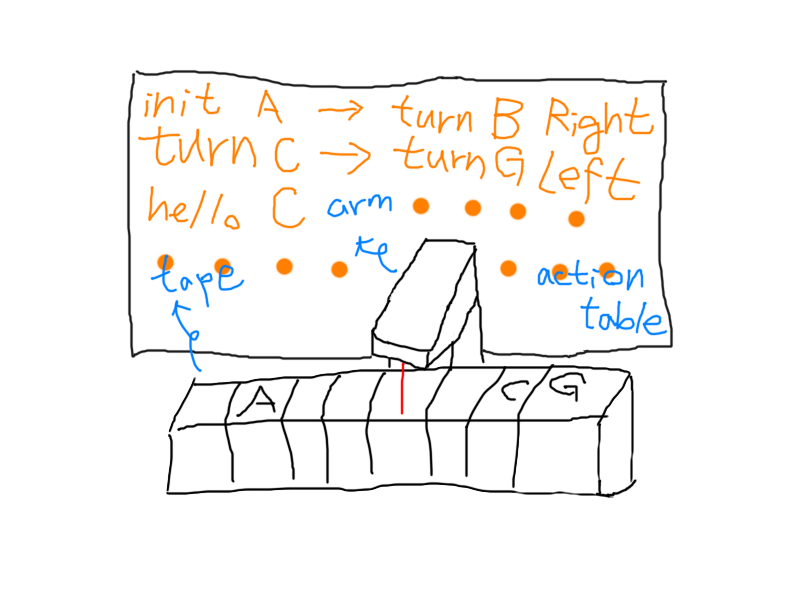
\includegraphics[width=1\textwidth]{image/turing-machine.png}
}

\frame{\frametitle{Turing Machine}
  \begin{itemize}
    \item<1->{\normalsize Infinite {\color{darkblue}tape} which stores symbols {\small(memory)}}
    \item<2->{\normalsize Finite {\color{darkblue}action table} which represents\\{\small (state, symbol) $\to$ action (program)}}
    \item<3->{\normalsize {\color{darkblue}Robotic arm} {\small (CPU with a register which stores current state)}
      \begin{itemize}
      \item<4->{\small Read the symbol on the tape at current position}
      \item<5->{\small Write a symbol on the tape at current position}
      \item<6->{\small Move the tape left or right}
      \end{itemize}
    }
  \end{itemize}
}

\ftc{Turing Complete}
\subsection{}
\ftc{So what is λ-calculus?}

\frame{\frametitle{Alligator Eggs!}
  \begin{figure}[h!]
    \centering
      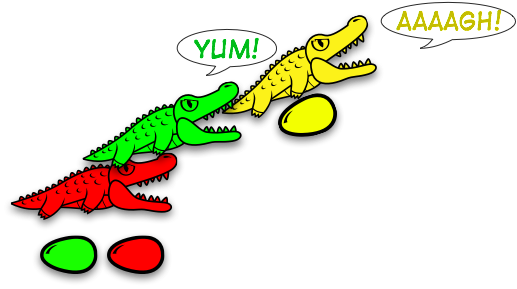
\includegraphics[width=0.85\textwidth]{image/eating.png}
      \caption{\jref{http://worrydream.com/AlligatorEggs/}{http://worrydream.com/AlligatorEggs/}}
  \end{figure}
}

\ftc{by Alonzo Church \\ in 1930s}
\ftc{Also Turing complete}
\ftc{but why?}
\subsection{λ-Complete}
\ftc{Define λ-Complete}
\ftc{Whatever λ-calculus can do}
\frame{\frametitle{Implement Turing machine in λ-calculus}
  \hskip 7mm
  \centering
  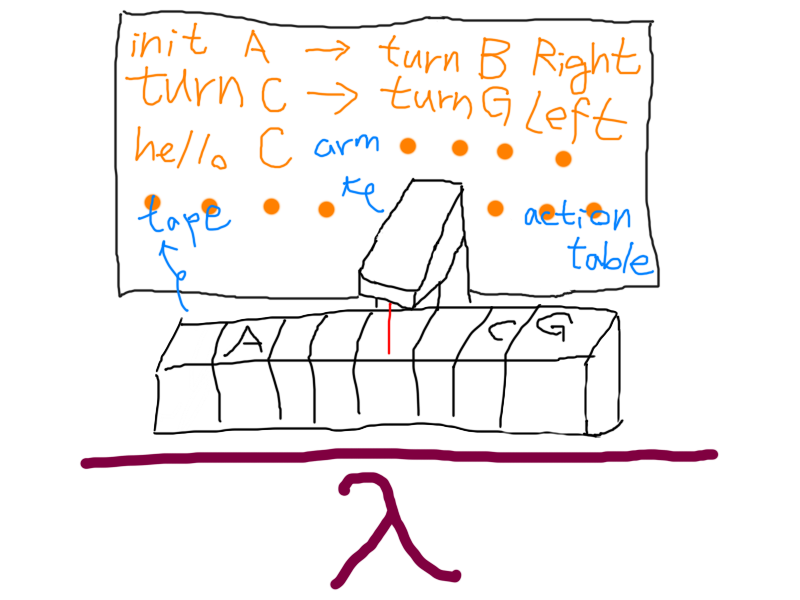
\includegraphics[width=0.85\textwidth]{image/turing-machine-lambda.png}
}
\frame{\frametitle{λ-Complete}
\begin{itemize}
  \item<1->{\normalsize So λ-calculus can do anything TM can do}
  \item<2->{\normalsize Plus what λ-calculus can do without a TM}
  \item<3->{\normalsize Thus λ-calculus is Turing complete}
\end{itemize}
}
\ftc{On the other hand...}
\frame{\frametitle{Implement λ-calculus in Turing machine}
  \hskip 7mm
  \centering
  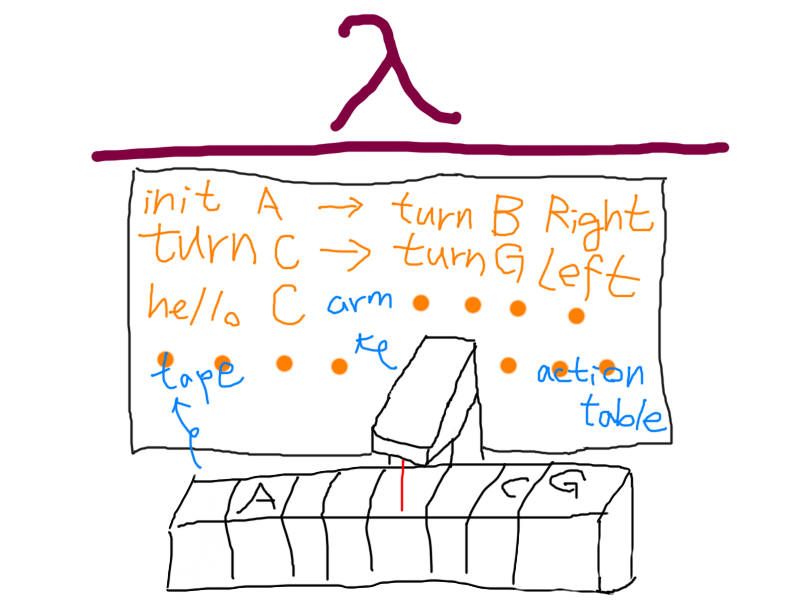
\includegraphics[width=0.85\textwidth]{image/lambda-turing-machine.png}
}
\ftc{So Turing machine is also λ-complete}
\frame{\frametitle{They have the same computability}
  \hskip 7mm
  \centering
  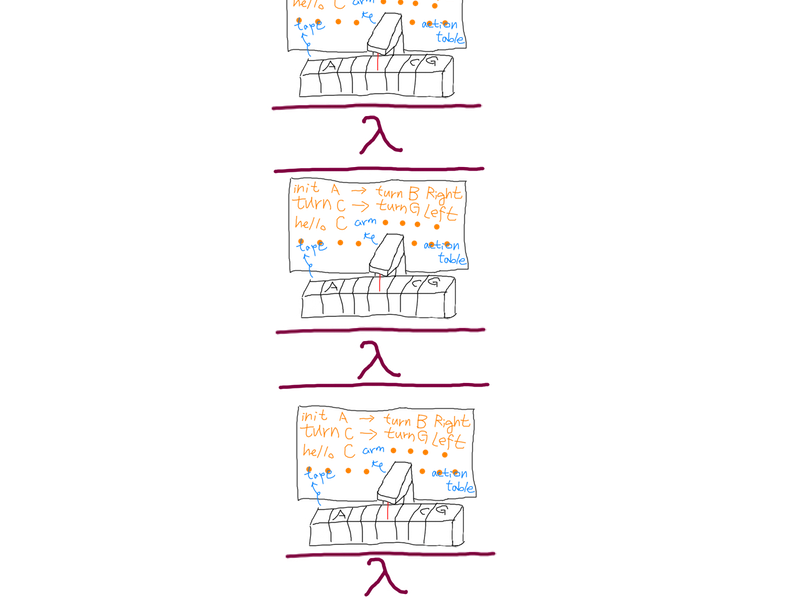
\includegraphics[width=0.85\textwidth]{image/inf.png}
}

\subsection{}

\frame{\frametitle{What exactly is λ-calculus?}
\begin{itemize}
  \item[]{}
  \item<1->{\usebeamerfont*{font DejaVu Sans Mono} (λx. x+1)}
  \item<2->{\usebeamerfont*{font DejaVu Sans Mono} (λx. x+1) 1}
  \item<3->{\usebeamerfont*{font DejaVu Sans Mono} = (1+1)}
  \item<4->{\usebeamerfont*{font DejaVu Sans Mono} = 2}
  \item[]{}
  \item[]{}
\end{itemize}
}

\frame{\frametitle{Does it look like Lisp?}
\begin{itemize}
  \item[]{}
  \item[]{}
  \item[]{\usebeamerfont*{font DejaVu Sans Mono} (λf.(λx.f (x x)) (λx.f (x x)))}
  \item[]{}
  \item[]{}
  \item[]{}
\end{itemize}
}

\subsection{Church Encoding}
\ftc{Church Encoding}

\frame{\frametitle{Natural Numbers}
\begin{itemize}
  \item[]{}
  \item{\usebeamerfont*{font DejaVu Sans Mono} 0 ≡ λf.λx. x}
  \item{\usebeamerfont*{font DejaVu Sans Mono} 1 ≡ λf.λx. f x}
  \item{\usebeamerfont*{font DejaVu Sans Mono} ...}
  \item{\usebeamerfont*{font DejaVu Sans Mono} n ≡ λf.λx. f$^{\text{n}}$ x}
  \item[]{}
\end{itemize}
}

\frame{\frametitle{Computation with Natural Numbers}
\begin{itemize}
  \item[]{}
  \item[]{}
  \item{\usebeamerfont*{font DejaVu Sans Mono} succ \ ≡ λn.λf.λx. f (n f x)}
  \item{\usebeamerfont*{font DejaVu Sans Mono} plus \ ≡ λm.λn.λf.λx. m f (n f x)}
  \item[]{}
  \item[]{}
\end{itemize}
}

\frame{\frametitle{Booleans}
\begin{itemize}
  \item[]{}
  \item[]{}
  \item{\usebeamerfont*{font DejaVu Sans Mono} true \ ≡ λa.λb. a}
  \item{\usebeamerfont*{font DejaVu Sans Mono} false ≡ λa.λb. b}
  \item[]{}
  \item[]{}
\end{itemize}
}

\frame{\frametitle{Computation with Booleans}
\begin{itemize}
  \item[]{}
  \item{\usebeamerfont*{font DejaVu Sans Mono} and \ \ ≡ λm.λn. m n m}
  \item{\usebeamerfont*{font DejaVu Sans Mono} or \ \ \ ≡ λm.λn. m m n}
  \item{\usebeamerfont*{font DejaVu Sans Mono} not \ \ ≡ λm.λa.λb. m b a}
  \item{\usebeamerfont*{font DejaVu Sans Mono} if \ \ \ ≡ λm.λa.λb. m a b}
  \item[]{}
\end{itemize}
}

\subsection{}

\frame{
\vskip 10mm%
\frametitlecenter{Recursion?\\No problems}
}

\subsection{Y combinator}

\frame{\frametitle{Y combinator}
\begin{itemize}
  \item[]{}
  \item<1->{Discovered by Haskell Curry}
  \item<1->{\normalsize\usebeamerfont*{font DejaVu Sans Mono} y \ \ = (λf.(λx.f (x x)) (λx.f (x x)))}
  \item<2->{\normalsize\usebeamerfont*{font DejaVu Sans Mono} y f = (λf.(λx.f (x x)) (λx.f (x x))) f}
  \item<3->{\normalsize\usebeamerfont*{font DejaVu Sans Mono} y f = f (y f)}
  \item[]{}
\end{itemize}
}

\frame{
\vskip 22mm%
\frametitlecenter{{\color{black} Paul Graham,}\\I know what is\\Y combinator!}
}

\subsection{Fixed Point Combinator}

\frame{\frametitle{Fixed Point Combinator}
\begin{itemize}
  \item[]{}
  \item{\normalsize Strict languages need some delay}
  \item{\footnotesize\usebeamerfont*{font DejaVu Sans Mono} Z = (λx.f (λv.((x x) v))) (λx.f (λv.((x x) v)))}
  \item{\normalsize Discovered by Alan Turing}
  \item{\footnotesize\usebeamerfont*{font DejaVu Sans Mono} Θ = (λx.λy. (y (x x y))) (λx.λy. (y (x x y)))}
  \item[]{}
\end{itemize}
}

\frame{\frametitle{Fixed Point Combinator}
\begin{itemize}
  \item[]{}
  \item{\normalsize Constructed by Jan Willem Klop}
  \item{\footnotesize\usebeamerfont*{font DejaVu Sans Mono} Yk = (L L L L L L L L L L L . . .)}
  \item[]{\tiny\usebeamerfont*{font DejaVu Sans Mono} where L = λabcdefghijklmnopqstuvwxyzr. (r (thisisafixedpointcombinator))}
  \item[]{}
  \item[]{}
\end{itemize}
}

\ftc{title}\frame{
\begin{itemize}
\item ...
\item ...
\item ...
\end{itemize}
}


\section{Let's Implement λ-Calculus}
\subsection{}

\frame{\frametitle{\color{white} dummy}
  \begin{itemize}
    \item {\color{lightgray} What can Haskell do?}
    \item {\color{lightgray} What is λ-Calculus?}
    \item {\color{lightgray} Why Implement λ-Calculus?}
    \item {Let's Implement λ-Calculus}
    \item {\color{lightgray} Questions?}
    \item {\color{lightgray} References}
  \end{itemize}
}

\frame{\frametitle{First Expression and evaluate (\jref{https://github.com/godfat/sandbox/blob/master/haskell/fpug/01/00.lhs
}{source})}
\footnotesize
\usebeamerfont*{font DejaVu Sans Mono}
module Main where \\
\color{white}. \\
data Expression = Literal Integer \\
 \ \ \ \ \ \ \ \ \ \ \ \ \ \ \ \ | Plus Expression Expression \\
{\color{white}.} \\
evaluate :: Expression -> Integer \\
evaluate (Literal i) \ \ \ \ \ \ \ = i \\
evaluate (Plus expr0 expr1) = \\
 \ \ evaluate expr0 + evaluate expr1 \\
{\color{white}.} \\
test0 = evaluate (Literal 1) \\
test1 = evaluate (Plus (Literal 1) (Literal 2)) \\
test2 = evaluate (Plus (Plus (Literal 1) \\
 \ \ \ \ \ \ \ \ \ \ \ \ \ \ \ \ \ \ \ \ \ \ \ \ \ \ \ \ \ (Literal 2)) \\
 \ \ \ \ \ \ \ \ \ \ \ \ \ \ \ \ \ \ \ \ \ \ \ (Literal 3))
}

\frame{\frametitle{First Expression and evaluate (\jref{https://github.com/godfat/sandbox/blob/master/haskell/fpug/01/00.lhs
}{source})}
\footnotesize
\usebeamerfont*{font DejaVu Sans Mono}
module Main where \\
{\color{white}.} \\
data Expression = Literal Integer \\
 \ \ \ \ \ \ \ \ \ \ \ \ \ \ \ \ | Plus Expression Expression \\
\color{white}. \\
evaluate :: Expression -> Integer \\
evaluate (Literal i) \ \ \ \ \ \ \ = i \\
evaluate (Plus expr0 expr1) = \\
 \ \ evaluate expr0 + evaluate expr1 \\
{\color{white}.} \\
test0 = evaluate (Literal 1) \\
test1 = evaluate (Plus (Literal 1) (Literal 2)) \\
test2 = evaluate (Plus (Plus (Literal 1) \\
 \ \ \ \ \ \ \ \ \ \ \ \ \ \ \ \ \ \ \ \ \ \ \ \ \ \ \ \ \ (Literal 2)) \\
 \ \ \ \ \ \ \ \ \ \ \ \ \ \ \ \ \ \ \ \ \ \ \ (Literal 3))
}

\frame{\frametitle{First Expression and evaluate (\jref{https://github.com/godfat/sandbox/blob/master/haskell/fpug/01/00.lhs
}{source})}
\footnotesize
\usebeamerfont*{font DejaVu Sans Mono}
module Main where \\
{\color{white}.} \\
data Expression = Literal Integer \\
 \ \ \ \ \ \ \ \ \ \ \ \ \ \ \ \ | Plus Expression Expression \\
{\color{white}.} \\
evaluate :: Expression -> Integer \\
evaluate (Literal i) \ \ \ \ \ \ \ = i \\
evaluate (Plus expr0 expr1) = \\
 \ \ evaluate expr0 + evaluate expr1 \\
\color{white}. \\
test0 = evaluate (Literal 1) \\
test1 = evaluate (Plus (Literal 1) (Literal 2)) \\
test2 = evaluate (Plus (Plus (Literal 1) \\
 \ \ \ \ \ \ \ \ \ \ \ \ \ \ \ \ \ \ \ \ \ \ \ \ \ \ \ \ \ (Literal 2)) \\
 \ \ \ \ \ \ \ \ \ \ \ \ \ \ \ \ \ \ \ \ \ \ \ (Literal 3))
}

\frame{\frametitle{First Expression and evaluate (\jref{https://github.com/godfat/sandbox/blob/master/haskell/fpug/01/00.lhs
}{source})}
\footnotesize
\usebeamerfont*{font DejaVu Sans Mono}
module Main where \\
{\color{white}.} \\
data Expression = Literal Integer \\
 \ \ \ \ \ \ \ \ \ \ \ \ \ \ \ \ | Plus Expression Expression \\
{\color{white}.} \\
evaluate :: Expression -> Integer \\
evaluate (Literal i) \ \ \ \ \ \ \ = i \\
evaluate (Plus expr0 expr1) = \\
 \ \ evaluate expr0 + evaluate expr1 \\
{\color{white}.} \\
test0 = evaluate (Literal 1) \\
test1 = evaluate (Plus (Literal 1) (Literal 2)) \\
test2 = evaluate (Plus (Plus (Literal 1) \\
 \ \ \ \ \ \ \ \ \ \ \ \ \ \ \ \ \ \ \ \ \ \ \ \ \ \ \ \ \ (Literal 2)) \\
 \ \ \ \ \ \ \ \ \ \ \ \ \ \ \ \ \ \ \ \ \ \ \ (Literal 3))
}

\frame{\frametitle{Algebraic Datatypes}
\footnotesize
\usebeamerfont*{font DejaVu Sans Mono}
{\color{white} module Main where \\
.} \\
data Expression = Literal Integer \\
 \ \ \ \ \ \ \ \ \ \ \ \ \ \ \ \ | Plus Expression Expression \\
{\color{white}. \\
evaluate :: Expression -> Integer \\
evaluate (Literal i) \ \ \ \ \ \ \ = i \\
evaluate (Plus expr0 expr1) = \\}
\usebeamerfont*{font DejaVu Sans} {\color{darkblue} Think of interface and subclasses if you like OOP} \\
\usebeamerfont*{font DejaVu Sans Mono} \color{white} . \\
test0 = evaluate (Literal 1) \\
test1 = evaluate (Plus (Literal 1) (Literal 2)) \\
test2 = evaluate (Plus (Plus (Literal 1) \\
\ \ \ \ \ \ \ \ \ \ \ \ \ \ \ \ \ \ \ \ \ \ \ \ \ \ \ \ \ (Literal 2)) \\
\ \ \ \ \ \ \ \ \ \ \ \ \ \ \ \ \ \ \ \ \ \ \ (Literal 3))
}

\frame{\frametitle{Pattern Matching}
\footnotesize
\usebeamerfont*{font DejaVu Sans Mono}
{\color{white} module Main where \\
.} \\
data Expression = Literal Integer \\
 \ \ \ \ \ \ \ \ \ \ \ \ \ \ \ \ | Plus Expression Expression \\
{\color{white}.} \\
evaluate :: Expression -> Integer \\
evaluate (Literal i) \ \ \ \ \ \ \ = i \\
evaluate (Plus expr0 expr1) = \\
 \ \ evaluate expr0 + evaluate expr1 \\
{\color{white}. \\
test0 = evaluate (Literal 1)} \\
\usebeamerfont*{font DejaVu Sans} {\color{darkblue} Think of dynamic\raisebox{.5mm}{\underline{ }}cast or instanceof with a switch if you like OOP} \\
\usebeamerfont*{font DejaVu Sans Mono} \color{white} test2 = evaluate (Plus (Plus (Literal 1) \\
 \ \ \ \ \ \ \ \ \ \ \ \ \ \ \ \ \ \ \ \ \ \ \ \ \ \ \ \ \ (Literal 2)) \\
 \ \ \ \ \ \ \ \ \ \ \ \ \ \ \ \ \ \ \ \ \ \ \ (Literal 3))
}

\frame{\frametitle{First Expression and evaluate (\jref{https://github.com/godfat/sandbox/blob/master/haskell/fpug/01/00.lhs
}{source})}
\footnotesize
\usebeamerfont*{font DejaVu Sans Mono}
module Main where \\
{\color{white}.} \\
data Expression = Literal Integer \\
 \ \ \ \ \ \ \ \ \ \ \ \ \ \ \ \ | Plus Expression Expression \\
{\color{white}.} \\
evaluate :: Expression -> Integer \\
evaluate (Literal i) \ \ \ \ \ \ \ = i \\
evaluate (Plus expr0 expr1) = \\
 \ \ evaluate expr0 + evaluate expr1 \\
{\color{white}.} \\
test0 = evaluate (Literal 1) \\
test1 = evaluate (Plus (Literal 1) (Literal 2)) \\
test2 = evaluate (Plus (Plus (Literal 1) \\
 \ \ \ \ \ \ \ \ \ \ \ \ \ \ \ \ \ \ \ \ \ \ \ \ \ \ \ \ \ (Literal 2)) \\
 \ \ \ \ \ \ \ \ \ \ \ \ \ \ \ \ \ \ \ \ \ \ \ (Literal 3))
}

\frame{\frametitle{Variable and Environment (\jref{https://github.com/godfat/sandbox/blob/master/haskell/fpug/01/01.lhs
}{source})}
\vskip -2.6mm%
\footnotesize
\usebeamerfont*{font DejaVu Sans Mono}
module Main where \\
{\color{white}.} \\
data Expression = Literal Integer \\
 \ \ \ \ \ \ \ \ \ \ \ \ \ \ \ \ | Plus Expression Expression \\
 \ \ \ \ \ \ \ \ \ \ \ \ \ \ \ \ | Variable String \\
\color{white}. \\
type Environment = [(String, Integer)] \\
\color{white}. \\
evaluate :: Expression -> Environment -> Integer \\
evaluate (Literal i) \ \ \ \ \ \ \ env = i \\
evaluate (Plus expr0 expr1) env = \\
 \ \ evaluate expr0 env + evaluate expr1 env \\
evaluate (Variable name) \ \ \ env = \\
 \ \ case lookup name env of (Just i) -> i
}

\frame{\frametitle{Variable and Environment (\jref{https://github.com/godfat/sandbox/blob/master/haskell/fpug/01/01.lhs
}{source})}
\vskip -2.6mm%
\footnotesize
\usebeamerfont*{font DejaVu Sans Mono}
module Main where \\
{\color{white}.} \\
data Expression = Literal Integer \\
 \ \ \ \ \ \ \ \ \ \ \ \ \ \ \ \ | Plus Expression Expression \\
 \ \ \ \ \ \ \ \ \ \ \ \ \ \ \ \ | Variable String \\
{\color{white}.} \\
type Environment = [(String, Integer)] \\
\color{white}. \\
evaluate :: Expression -> Environment -> Integer \\
evaluate (Literal i) \ \ \ \ \ \ \ env = i \\
evaluate (Plus expr0 expr1) env = \\
 \ \ evaluate expr0 env + evaluate expr1 env \\
evaluate (Variable name) \ \ \ env = \\
 \ \ case lookup name env of (Just i) -> i
}

\frame{\frametitle{Variable and Environment (\jref{https://github.com/godfat/sandbox/blob/master/haskell/fpug/01/01.lhs
}{source})}
\vskip -2.6mm%
\footnotesize
\usebeamerfont*{font DejaVu Sans Mono}
module Main where \\
{\color{white}.} \\
data Expression = Literal Integer \\
 \ \ \ \ \ \ \ \ \ \ \ \ \ \ \ \ | Plus Expression Expression \\
 \ \ \ \ \ \ \ \ \ \ \ \ \ \ \ \ | Variable String \\
{\color{white}.} \\
type Environment = [(String, Integer)] \\
{\color{white}.} \\
evaluate :: Expression -> Environment -> Integer \\
\color{white} evaluate (Literal i) \ \ \ \ \ \ \ env = i \\
evaluate (Plus expr0 expr1) env = \\
 \ \ evaluate expr0 env + evaluate expr1 env \\
evaluate (Variable name) \ \ \ env = \\
 \ \ case lookup name env of (Just i) -> i
}

\frame{\frametitle{Variable and Environment (\jref{https://github.com/godfat/sandbox/blob/master/haskell/fpug/01/01.lhs
}{source})}
\vskip -2.6mm%
\footnotesize
\usebeamerfont*{font DejaVu Sans Mono}
module Main where \\
{\color{white}.} \\
data Expression = Literal Integer \\
 \ \ \ \ \ \ \ \ \ \ \ \ \ \ \ \ | Plus Expression Expression \\
 \ \ \ \ \ \ \ \ \ \ \ \ \ \ \ \ | Variable String \\
{\color{white}.} \\
type Environment = [(String, Integer)] \\
{\color{white}.} \\
evaluate :: Expression -> Environment -> Integer \\
evaluate (Literal i) \ \ \ \ \ \ \ env = i \\
evaluate (Plus expr0 expr1) env = \\
 \ \ evaluate expr0 env + evaluate expr1 env \\
evaluate (Variable name) \ \ \ env = \\
 \ \ case lookup name env of (Just i) -> i
}

\frame{\frametitle{Variable and Environment (\jref{https://github.com/godfat/sandbox/blob/master/haskell/fpug/01/01.lhs
}{source})}
\vskip -2.6mm%
\footnotesize
\usebeamerfont*{font DejaVu Sans Mono}
test0 = evaluate (Variable "var") [("var", 1)] \\
test1 = evaluate (Plus (Variable "var") (Literal 2)) [("var", 1)]
}

\frame{\frametitle{Type Alias}
\vskip -2.6mm%
\footnotesize
\usebeamerfont*{font DejaVu Sans Mono}
module Main where \\
{\color{white}.} \\
data Expression = Literal Integer \\
 \ \ \ \ \ \ \ \ \ \ \ \ \ \ \ \ | Plus Expression Expression \\
 \ \ \ \ \ \ \ \ \ \ \ \ \ \ \ \ | Variable {\color{darkblue}Name} \\
{\color{white}.} \\
type {\color{darkblue}Name} = String \\
type Environment = [({\color{darkblue}Name}, Integer)] \\
{\color{white}.} \\
evaluate :: Expression -> Environment -> Integer \\
evaluate (Literal i) \ \ \ \ \ \ \ env = i \\
evaluate (Plus expr0 expr1) env = \\
 \ \ evaluate expr0 env + evaluate expr1 env \\
evaluate (Variable name) \ \ \ env = \\
 \ \ case lookup name env of (Just i) -> i
}
\frame{\frametitle{Pair}
\vskip -2.6mm%
\footnotesize
\usebeamerfont*{font DejaVu Sans Mono}
("var", 2) :: (String, Integer) \\
(2, "var") :: (Integer, String)
}

\frame{\frametitle{List}
\vskip -2.6mm%
\footnotesize
\usebeamerfont*{font DejaVu Sans Mono}
[1,2,3] :: [Integer] \\
["a","b","c"] :: [String] \\
("var", 1) :: [(String, Integer)]
}


\section{}
\subsection{}
\frame{\frametitle{We're hiring}
\begin{itemize}
  \item[]{}
  \item[]{}
  \item[]{
\includegraphics[width=0.5\textwidth]{image/cb.png}}
  \item[]{\jref{http://cblue.tw/jobs}{cblue.tw/jobs}}
  \item[]{}
  \item[]{}
\end{itemize}
}

\frame{\frametitle{Feel free to ask me questions online}
\begin{itemize}
\item[] {}
\item \jref{https://github.com/godfat}{github.com/godfat}
\item \jref{https://twitter.com/godfat}{twitter.com/godfat}
\item \jref{https://profiles.google.com/godfat}{profiles.google.com/godfat}
\item[] {}
\item[] {}
\end{itemize}
}


\section{}
\subsection{}
\frame{\frametitle{References}
\begin{itemize}
  \item{To be listed...}
  \item{}
  \item{}
  \item{}
  \item{}
  \item{}
\end{itemize}
}


\end{document}
